%%%%%%%%%%%%%%%%%%%%%%%%%%%%%%%%%%%%%%START PREAMBLE THAT IS THE SAME FOR ALL EXAMPLES
\documentclass{article}

%Required: You must have these
\usepackage{Sweave}
\usepackage{graphicx}
\usepackage{tabularx}
\usepackage{hyperref}
\usepackage{natbib}
\usepackage{pdflscape}
\usepackage{array}
\usepackage{gensymb}
\usepackage{authblk}
%\usepackage[backend=bibtex]{biblatex}
%Strongly recommended
  %put your figures in one place
%\SweaveOpts{prefix.string=figures/, eps=FALSE} 
%you'll want these for pretty captioning
\usepackage[small]{caption}

\setkeys{Gin}{width=0.8\textwidth}  %make the figs 50 perc textwidth
\setlength{\captionmargin}{30pt}
\setlength{\abovecaptionskip}{10pt}
\setlength{\belowcaptionskip}{10pt}
% manual for caption  http://www.dd.chalmers.se/latex/Docs/PDF/caption.pdf

%Optional: I like to muck with my margins and spacing in ways that LaTeX frowns on
%Here's how to do that
 \topmargin -1.5cm        
 \oddsidemargin -0.04cm   
 \evensidemargin -0.04cm  % same as oddsidemargin but for left-hand pages
 \textwidth 16.59cm
 \textheight 21.94cm 
 %\pagestyle{empty}       % Uncomment if don't want page numbers
 \parskip 7.2pt           % sets spacing between paragraphs
 %\renewcommand{\baselinestretch}{1.5} 	% Uncomment for 1.5 spacing between lines
\parindent 0pt% sets leading space for paragraphs
\usepackage{setspace}
%\doublespacing

%Optional: I like fancy headers
%\usepackage{fancyhdr}
%\pagestyle{fancy}
%\fancyhead[LO]{How do climate change experiments actually change climate}
%\fancyhead[RO]{2016}
 
%%%%%%%%%%%%%%%%%%%%%%%%%%%%%%%%%%%%%%END PREAMBLE THAT IS THE SAME FOR ALL EXAMPLES

%Start of the document
\begin{document}

%\SweaveOpts{concordance=TRUE}

\bibliographystyle{/Users/ailene.ettinger/Documents/GitHub/fishphen/refs/bibstyles/amnat.bst}% i moved a style file into the ospree git repo. feel free to add whatever style you like and update, lizzie! I don't have besjournals

\title{Soil moisture interacts with temperature to affect plant phenology}

\date{\today}
\maketitle %put the fancy title on
%\tableofcontents %add a table of contents

\author{A.K. Ettinger, J.S. Dukes, M.R. Johnston, C.R. Rollinson, E.M. Wolkovich}

%\textbf{Statement of authorship} 
%All authors conceived of this manuscript, which began at a Radcliffe Exploratory Seminar in 2016, and all authors contributed to manuscript revisions. AKE and EMW conceived of the idea for the literature review, database compilation, and related Radcliffe Exploratory Seminar. AKE compiled the datasets; AKE analyzed the data and created the figures.

\textbf{Data Accessibility} %Data accessibility statement: The statement must confirm that, should the manuscript be accepted, the data supporting the results will be archived in an appropriate public repository such as Dryad or Figshare and the data DOI will be included at the end of the article.
The data reported in this paper are from the MC3E and ExPhen databases, which are available at KNB \citep{ettinger2018,ettinger2019}

\textbf{Running title} Soil moisture affects phenology


\textbf{Key words} global warming, warming experiment, microclimate, phenology, bud-burst, leaf-out, flowering, fruiting, senescence 


\clearpage
%%%%%%%%%%%%%%%%%%%%%%%%%%%%%%%%%%%%%%%%%%%%%%%%%%%
\section*{Abstract}
Past studies of phenology responses to recent climate change have focused on temperature as a driver of observed shifts. However, soil moisture is also affected by climate change and likely to alter biological responses. Here we synthesize microclimate and phenology data from climate change experiments to show how soil moisture interacts with temperature to affect plant phenology. We find that soil drying generally delays delays plant phenology, especially for budburst, a rate of XX days per percent VWC, on average. These effects vary widely across sites and species. This rate suggests that, on average, climate change- induced shifts soil moisture will play only a small role in altering future phenology, compared to shifts in temperature. This is both because of the strong sensitivity of plant phenology to temperature and because of the large magnitude of projected shifts in temperature, compared to shifts in soil moisture. Nonetheless, although effects of soil moisture are comparably small on average, sensitivity to soil moisture varied dramatically by species, and soil moisture levels differed by site and among years. Thus, soil moisture is likely to play a role in phenological shifts with climate change for some species, at some sites and years. Quantifying phenological sensitivity to changes in soil moisture will be useful for improving forecasts of shifts in phenology with future climate change.  

\section* {Main text Outline}
\begin{enumerate}
\item Climate change is affecting organisms by altering temperature and soil moisture around the world \citep{parmesan2006,chen2010}. One of most widespread biological responses to climate change is a shift in phenology, the timing of recurring biological events, which has occurred at rates of 2.3-5.1 days per decade \citep{parmesan2006,poloczanska2013,root2003}.
\item Phenological shifts are typically attributed to warming temperature.
\item Soil moisture may also shift with climate change; effects of altered soil moisture on phenology have received less attention, but are likely to be important drivers of plant phenology. 
\begin{enumerate}
\item Effects of water in dry ecosystems \citep{essiamah1986,reich1984, van1993}. 
\item Budburst can be slowed by water stress through inhibiting cell elongation \citep{essiamah1986}, and growing season start may be delayed by drought in grasslands \cite{cui2017}. 
\item Flowering phenology can be advanced by drought conditions \citep{hamann2018}. 
\end{enumerate}
\item Here we conduct a meta-analyses of climate change experiments to test whether and how soil moisture interacts with temperature to affect plant phenology. Previous meta-analyses of phenology in climate change experiments have focused primarily on effects of temperature \citep{wolkovich2012}. 
\begin{enumerate}
\item We expected that soil moisture may also affect phenology, with drier soils delaying budburst and leafout phenology and advancing flowering and fruiting phenology.  
\item We use measured microclimate and phenology data from two databases of climate change experiments: MicroClimate from Climate Change Experiments (MC3E) and Experimental Phenology (ExPhen)  to quantify effects of soil moisture and above-ground temperature on plant phenology (bud-burst, leaf-out, flowering, fruiting, senescence; see Methods). 
\item We also use forecasted changes in temperature and soil moisture to investigate how including soil moisture alters expected future shifts in phenology. 
\end{enumerate}
\item We find that soil drying delays phenology and warming temperatures advance phenology, for most phenophases. Soil drying delays spring budburst at a rate of 0.42 days per percent reduction in soil VWC. Increasing air temperature advanced phenology for all phenophases except senescence (Figure 2S). Warming advances budburst phenology at a rate of 3.42 days per \degree C, a rate that is consistent with estimates from previous meta-analyses \citep{wolkovich2012}. The magnitude of soil moisture effects varies with temperature, though not strongly (Figure \ref{fig:smtempbb}). Effects of soil moisture also varies across phenophases and species.  

\item The effect of soil moisture varies by species: \emph{Magnolia grandiflora} and \emph{Carya glabra} had the strongest negative effects of soil moisture; \emph{Betula alleghaniensis} and \emph{B. populifolia} had positive effects of soil moisture (perhaps because they occur at the site where snowfall is greatest- Harvard? More moisture= more recent snowmelt = delayed phenology?)
\item Effects of soil moisture were strongest for budburst and leafout, and affected all phenophases, except fruiting (Figures \ref{fig:modests}, 2S), to varying degrees. 
\begin{enumerate}
\item Different phenophases require different physiological pathways, so it makes sense that they would respond differently to changes in soil moisture. 
\item In addition, the relationship between soil moisture and temperature varies seasonally. Soil moisture and temperature are correlated, especially in control plots (Figure \ref{fig:site}). Temperature and soil moisture were more strongly related in treatment plots later in the year (April-June), than earlier in the year (Jan-Mar). 
\end{enumerate}
\item Relationships between above-ground temperature and soil moisture vary widely by site, likely becuase of differences in experimental design, as well as soil type and other factors. These differences may alter the effects of microcliamte on phenology, as well, but were not able to include site-level differences in the effects of soil moisture and temperature on phenology, because parameters were not estimable with this added model complexity. (Though we did account for site-level differences on the intercept.)
\item Although soil moisture affects phenology for all phenophases we studied, we find that soil moisture is unlikely to dramatically alter the timing of budburst in the future. 
\begin {enumerate}
\item This is both because temperature has a stronger effect on phenology and because temperature is expected to shift more dramaticly than soil moisture.
\item Although forecasted changes in soil moisture are unlikely to dramatically later phenology, on average, site and species variation is great so it may be important in some locations, for some species. 

\end{enumerate}
\end{enumerate}


\section* {Figures}

 \begin{figure}[h]
\centering
 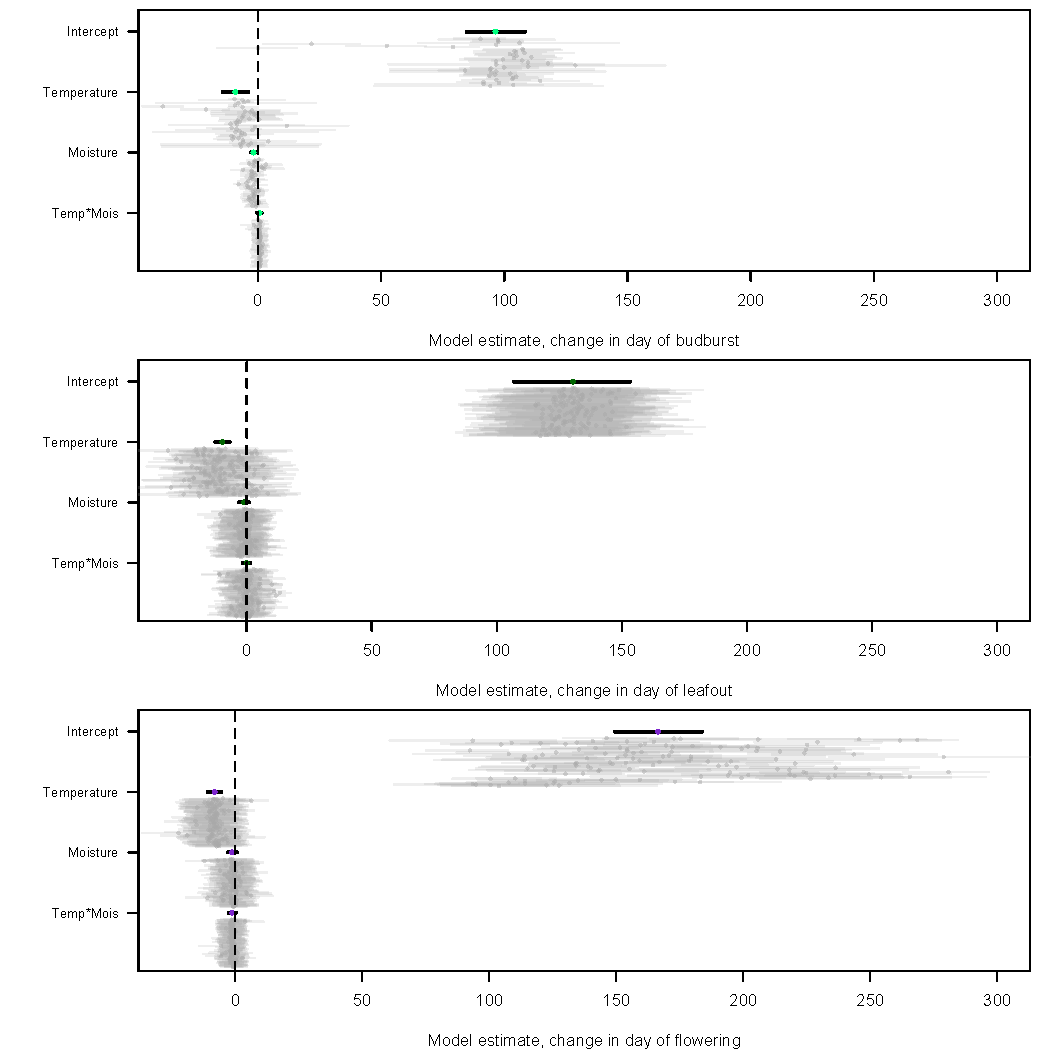
\includegraphics{/Users/ailene.ettinger/Documents/GitHub/radcliffe/Analyses/soilmoisture/figures/m5bbdlodffd.pdf}
 \caption{Model estimates of effects of of above-ground temperature and soil moisture on budburst (top panel), leafout (middle panel) and flowering (bottom panel).} 
 \label{fig:modests}
 \end{figure}
\begin{figure}[h]
\centering
 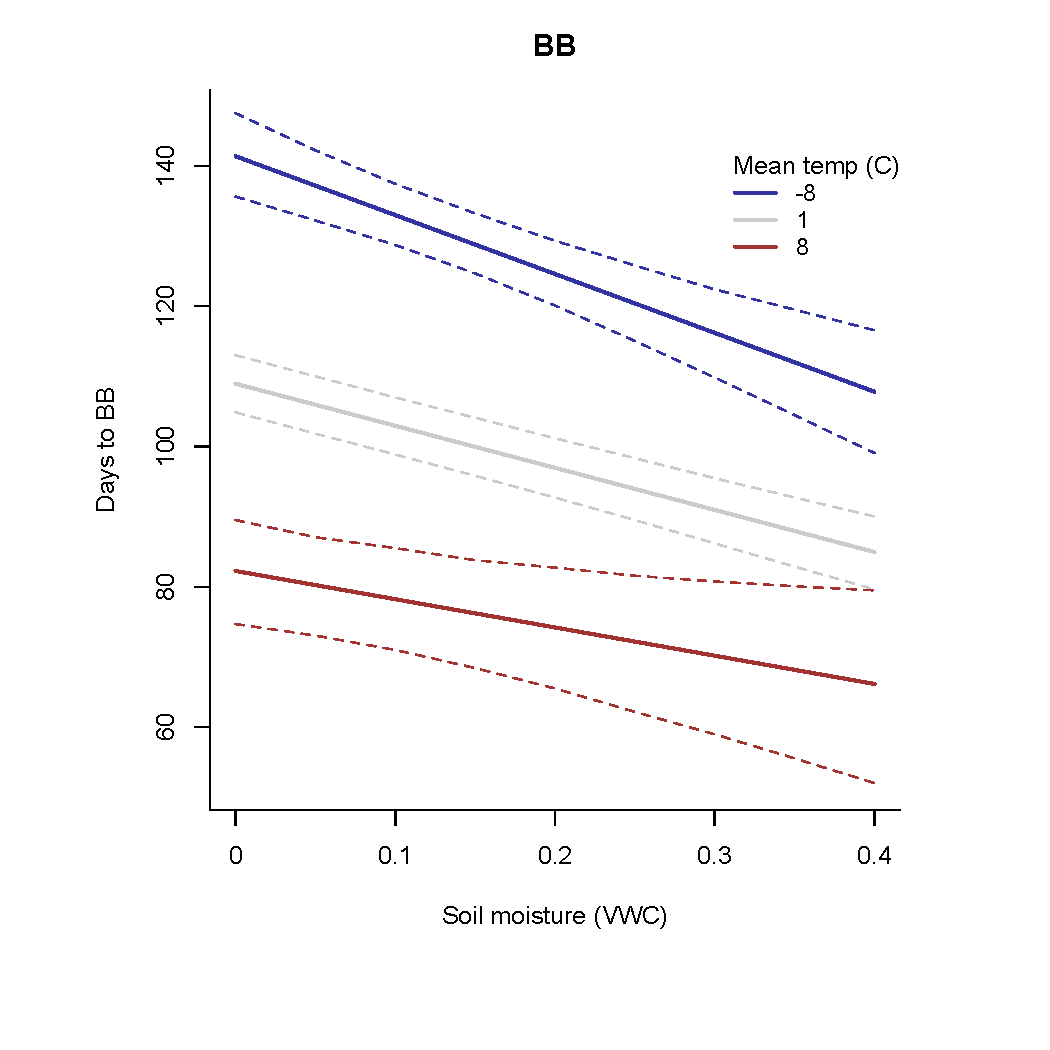
\includegraphics{/Users/ailene.ettinger/Documents/GitHub/radcliffe/Analyses/soilmoisture/figures/soilmois_apc.pdf}
 \caption{The effect of soil moisture varies slightly with temperature, for budburst.} 
 \label{fig:smtempbb}
 \end{figure}

\begin{figure}[h]
\centering
 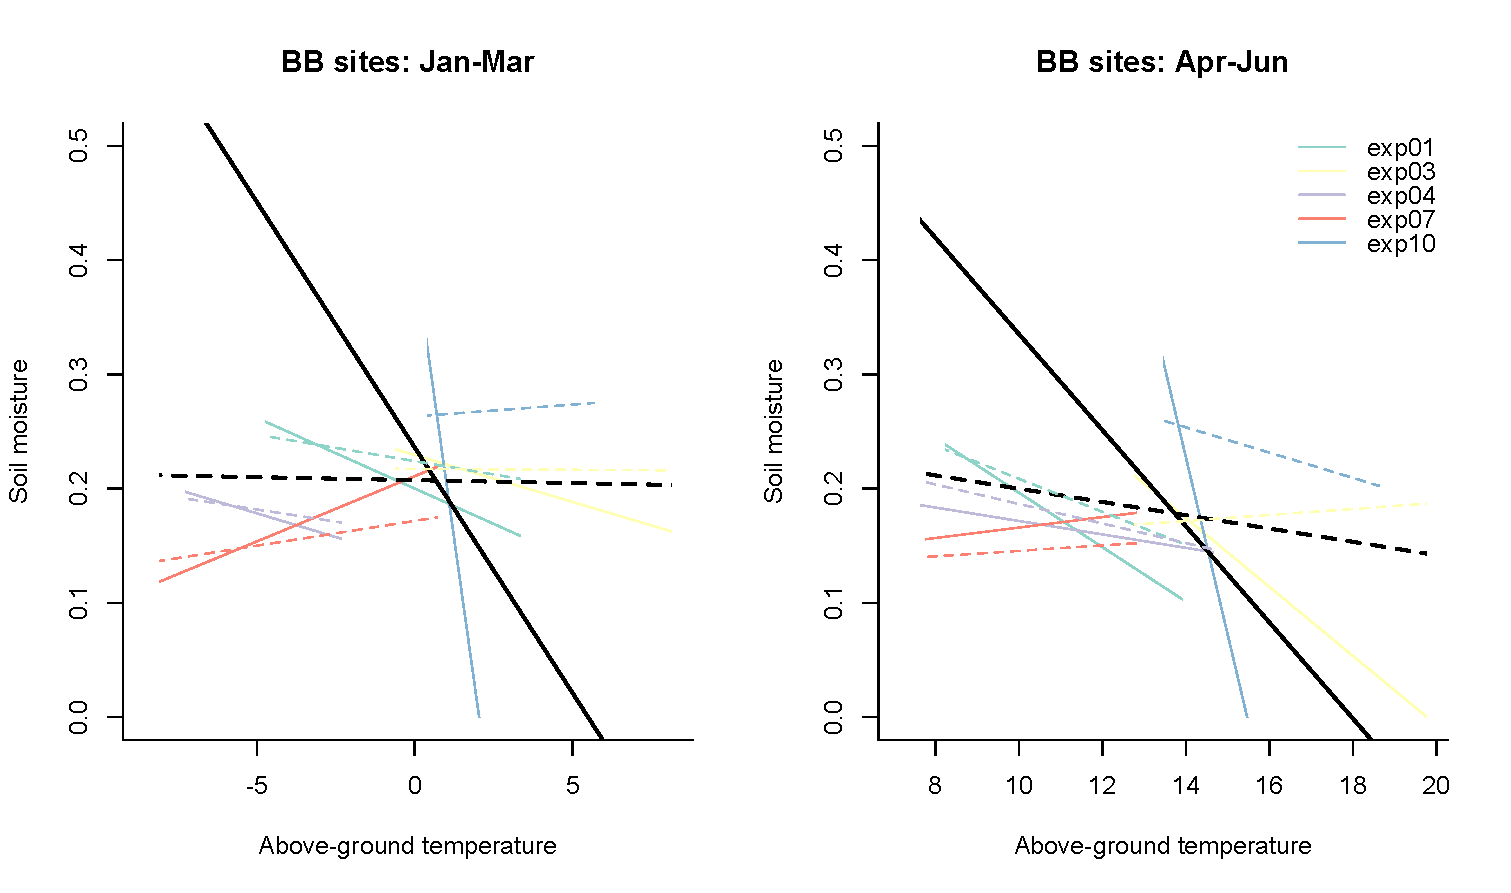
\includegraphics{/Users/ailene.ettinger/Documents/GitHub/radcliffe/Analyses/figures/smtemosum_bysite.pdf}
 \caption{The relationship between soil moisture and temperature is different in treatment and control plots, and this relationship varies by site and time of year.} 
 \label{fig:site}
 \end{figure}

\begin{figure}[h]
\centering
 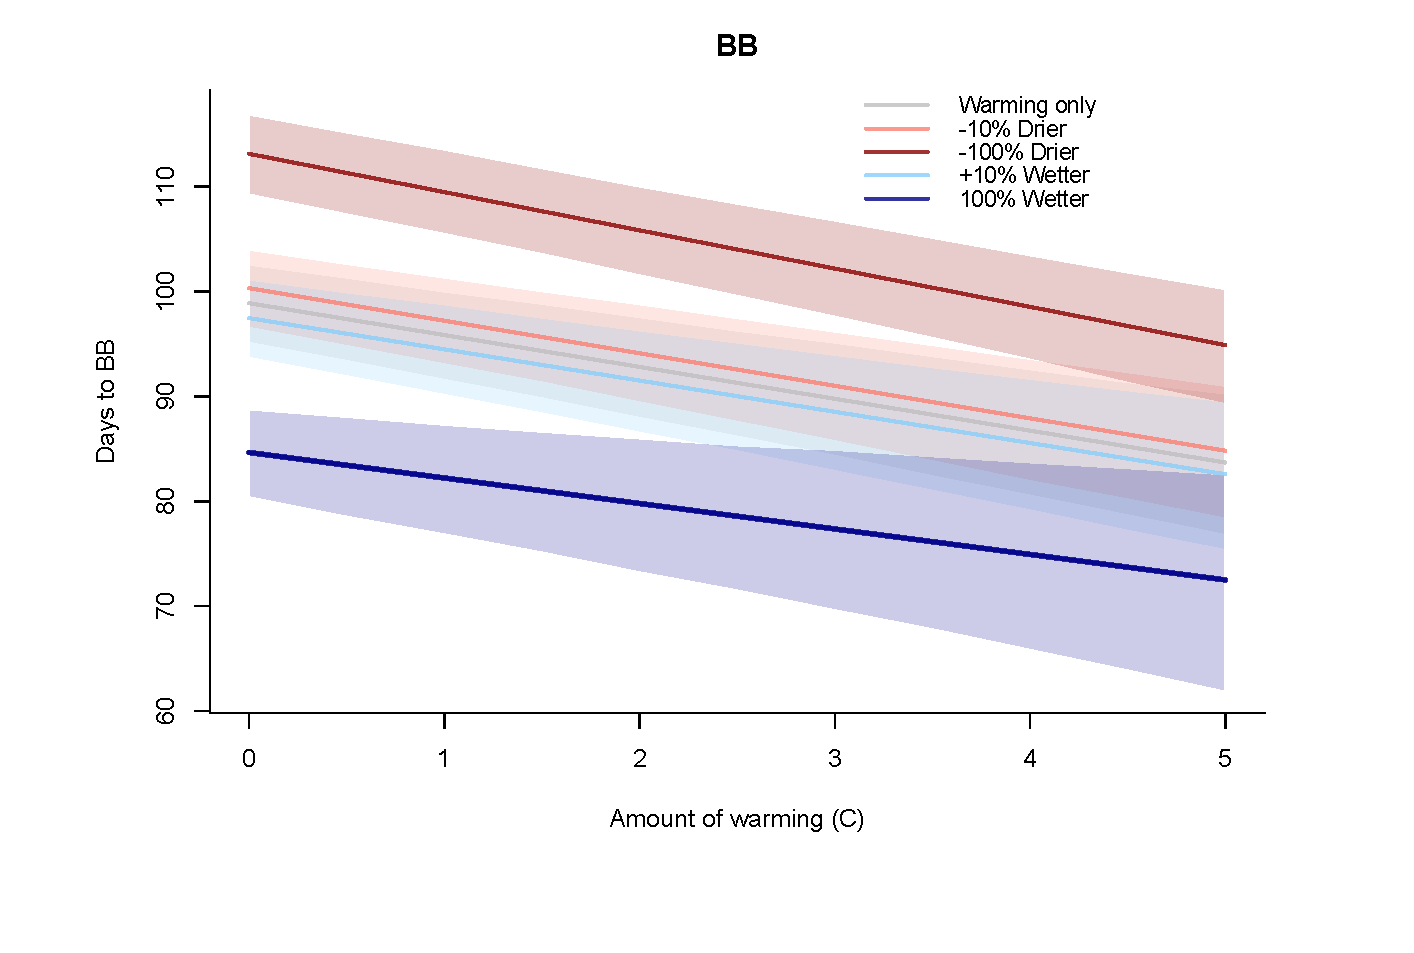
\includegraphics{/Users/ailene.ettinger/Documents/GitHub/radcliffe/Analyses/soilmoisture/figures/bbmod_forecast_uncent_wCI.pdf}
 \caption{Expected effect of soil moisture on budburst, at different amounts of forecasted warming.} 
 \label{fig:forecast}
 \end{figure}
 
\clearpage
\bibliography{/Users/ailene.ettinger/Documents/citations/Bibtex/mylibrary.bib}

\section* {Methods}
\underline{Data}: 
\par To investigate how soil moisture interacts with temperature to affect phenology, we used two databases that compile data from climate change experiments. Microclimate data came from the  MicroClimate from Climate Change Experiments (MC3E) database \cite{ettinger2018}. Phenology data came from a ExPhen, a new database of phenology from climate change experiments \cite{ettinger2018b}. 
\par To create both databases, we first identified published, active-warming field experiments, many of which included precipitation manipulations. We focused on \textit{in situ} active-warming manipulations because recent analyses indicate that active-warming methods are the most controlled and consistent methods available for experimental warming \citep{kimball2005,kimball2008,aronson2009,wolkovich2012}. We carried out a full literature review to identify potential active-warming field experiments, following the methods and search terms of \citet{wolkovich2012} for their Synthesis of Timings Observed in iNcrease Experiments (STONE) database \citep{wolkovich2012}, but restricting our focus to active-warming experiments. Further, because our goal was to tease out variation in microclimate (including temperature and soil moisture), we focused on warming studies that included both/either multiple levels of warming and/or precipitation treatments. These additional restrictions constrained the list to 11 new studies published after the STONE database, as well as six of the 37 studies in the STONE database. We contacted authors to obtain daily microclimate and phenological data for these 17 studies and received data (or obtained publicly available data) for 10 of them, as well as datasets from five additional sites offered or suggested to us over the course of our literature review and data analysis. The daily temperature and soil moisture data from these 15 experiments comprise the MC3E database, which is available at KNB \citep{ettinger2018}. The phenology data from the same 15 experiments comprise the ExPhen database of experimental phenology, which is also available at KNB \citep{ettinger2018b}.

\underline{Analysis}:

\par To understand how soil moisture interacts with temperature to affect phenology, we fit models with measured soil moisture, measured temperature, and their interaction to phenology response data (budburst, leafout, flowering, fruiting, senescence). Microclimate data came from the MC3E database, and phenology data came from the ExPhen database. We excluded conifers from the analysis, because their phenology has distinct differences from angiosperm phenology \cite{polgar2014} and conifer data existed from only one site in the database. For all phenology variables, the response variable was day-of-year of the phenological event. Predictors for our primary models were measured air temperature, soil moisture, and their interaction. We also fit model(s) with soil temperature in place of air temperature. Random effects for all phenology models were species (with random slopes and intercepts), site (random intercept), and year nested within site (random intercept). Equations for these models can be found in the Supplemental Methods. 
To better understand the interactive effects of measured temperature and soil moisture, we conducted follow-up analyses in which we fit the same phenology models subsets of the data (controls only, low temperature treatments only, and high temperature treatments only).
\par To quantify how climate manipulations affect temperature and soil moisture, we used microclimate data from the 4 sites in the MC3E database that manipulated both precipitation and temperature, and measured both above-ground temperature and soil moisture data (exp01,exp05,exp07,exp12). (OR use all 8 studies that measured soil moisture and above-ground temp?) We then fit two groups of hierarchical models to microclimate data from these sites: one group with temperature response variables (including mean annual, and mean seasonal temperatures), and the other group with soil moisture as response variables (including mean annual, and mean seasonal soil moisture). For both groups of models, explanatory variables were temperature treatment, precipitation treatment, and their interaction. The models included a random effect of site, with a random slope and intercept structure, to allow effects of experimental treatments to vary across sites. Models also included random effects of day-of-year, nested within year, on the intercept only, to account for non-independence of measurements taken on the same day within the same year. Equations for these models can be found in the Supplemental Methods. 

\section* {Supplemental Figures}
 \begin{figure}[h]
\centering
 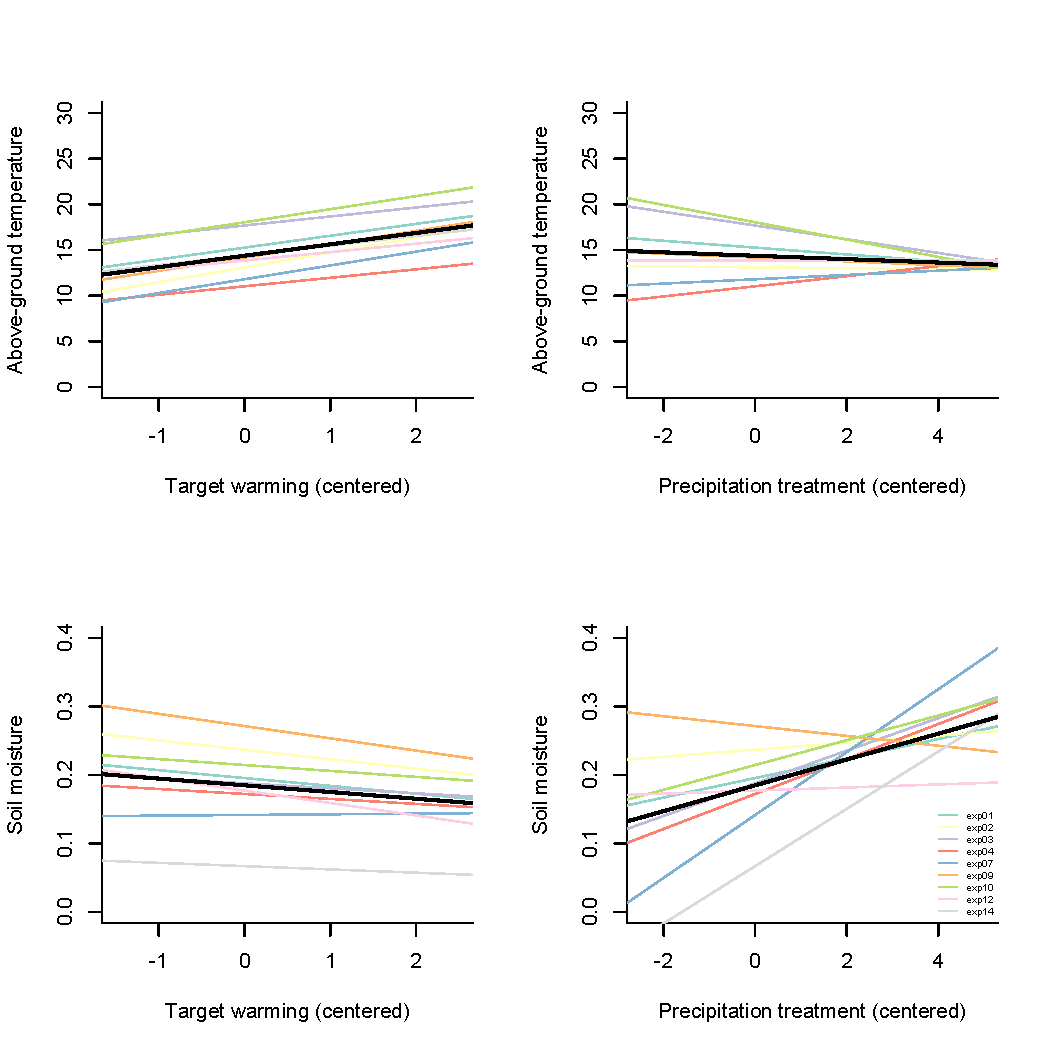
\includegraphics{/Users/ailene.ettinger/Documents/GitHub/radcliffe/Analyses/soilmoisture/figures/smtempvstargtemppreciptreat_lineslmerALL.pdf}
 \caption{Effects of target temperature and precipitation treatments on above-ground temperature and soil moisture.} 
 \label{fig:soilmois}
 \end{figure}

Figure 2S: Model Estimates for fruiting and senescence.

\end{document}
